\documentclass[UTF8,a4paper,11pt]{ctexart}

\usepackage[margin=2.3cm]{geometry}
\usepackage{graphicx}
\usepackage{booktabs}
\usepackage{array}
\usepackage{float}
\usepackage{xcolor}
\usepackage{hyperref}
\usepackage{enumitem}
\usepackage{caption}
\usepackage{amsmath}

\hypersetup{
  colorlinks=true,
  linkcolor=blue!50!black,
  urlcolor=blue!55!black,
  citecolor=blue!50!black
}

\setlength{\parindent}{2em}
\setlength{\parskip}{0.25em}
\setlist[itemize]{itemsep=0.15em, topsep=0.2em}
\setlist[enumerate]{itemsep=0.15em, topsep=0.2em}
\captionsetup{font=small, labelfont=bf}

\title{\textbf{作业三：真实三维场景的多表示重建与评估}}
\author{
  姓名：\underline{\hspace{3cm}} \quad
  学号：\underline{\hspace{3cm}} \quad
  班级：\underline{\hspace{3cm}}
}
\date{\today}

\begin{document}

\maketitle

\begin{abstract}
本文围绕同一真实静态讲台场景，对三种三维表示进行重建与评估：COLMAP 稀疏几何、Nerfacto/NeRF 隐式辐射场，以及官方 3D Gaussian Splatting 显式辐射基元。实验数据来自自行拍摄的视频，抽帧后得到 51 张图像，其中 46 张作为训练视角，5 张作为预留测试视角。实验重点不是单纯追求最清晰的渲染，而是比较不同表示学到了什么、丢掉了什么，以及在视觉质量、几何质量、效率、可编辑性和适用场景上的差异。

结果显示，COLMAP 能恢复稳定的相机轨迹和可用的稀疏点云，训练集 46 张图像全部注册，平均重投影误差为 0.945 px，但低纹理墙面和反光桌面区域点云稀疏。Nerfacto 的新视角指标为 PSNR 19.18、SSIM 0.767、LPIPS 0.371，能够恢复整体结构，但在边界、细线缆和低纹理区域出现模糊与漂浮伪影。3DGS 在可获得的 hold-out 渲染上达到 PSNR 24.59、SSIM 0.817、LPIPS 0.177，外观更锐利、训练和渲染更快，但其 Gaussian 分布仍不等价于真实表面几何。综合来看，COLMAP 更适合作为位姿和稀疏几何基线，NeRF 更强调连续隐式场表示，3DGS 在本实验场景中取得了最好的外观质量和效率折中。
\end{abstract}

\section{数据采集与预处理}

\subsection{场景与采集方式}

实验场景为一处真实室内讲台区域，包含讲台桌面、椅子、黑板、墙面、门框、电源线、显示器支架等结构。该场景整体静态，便于从不同视角采集图像并进行多视角重建。原始数据为自行拍摄视频 \texttt{data/raw/desk.mp4}，视频长度约 25.21 s，OpenCV 读取分辨率为 $720 \times 1280$，帧率约 29 FPS。

预处理脚本从视频中抽取 51 张图像，并统一使用同一份图像集合进行后续位姿估计、神经渲染训练和 Gaussian Splatting 训练。根据项目配置，实验保留约 10\% 图像作为测试视角：训练集包含 46 张，测试集包含 5 张。抽帧、划分和路径记录均保存在项目脚本与结果目录中，避免不同方法使用不同数据口径。

\subsection{相机参数与位姿来源}

视频抽帧后没有保留完整的手机 EXIF 标定信息，因此本文不把手机出厂参数作为相机真值。所有方法使用的可复现实验相机参数来自 COLMAP/SfM 估计。全量图像的 COLMAP 模型注册 51 张图像并恢复 2590 个稀疏三维点；训练集模型注册 46 张图像并恢复 2113 个稀疏三维点。训练集估计相机模型为 SIMPLE\_RADIAL，焦距约 1103.76 像素，主点为 $(360, 640)$，径向畸变参数约 0.0512。

需要强调的是，COLMAP 输出是估计几何，而不是绝对真值。本文将其作为相机位姿来源和几何基线，不用它直接替代真实世界三维结构。

\section{三种三维表示方法}

\subsection{COLMAP 稀疏几何}

COLMAP 使用特征提取、穷举匹配、增量式 SfM 和 bundle adjustment，从多视角图像中估计相机位姿、共享相机内参和稀疏三维点。其表示形式是显式的稀疏点云和相机轨迹。该方法几何解释性强，但依赖可匹配纹理；在墙面、反光桌面和重复纹理区域容易缺点或产生离群点。

在本实验中，COLMAP 的作用有两层：第一，作为传统几何基线，用于分析相机轨迹和稀疏点云质量；第二，作为 Nerfacto 和 3DGS 的位姿初始化来源。训练集点云平均重投影误差为 0.945 px，中位数为 0.847 px，平均 track length 为 3.995，说明多视角匹配整体稳定，但点云仍明显稀疏。

\subsection{Nerfacto / NeRF}

Nerfacto 属于连续隐式辐射场表示。它通过神经网络学习空间位置和观察方向到颜色、密度等渲染量的映射，并通过体渲染生成新视角图像。与稀疏点云相比，NeRF 不直接存储显式曲面，而是通过密度场隐式表达几何和外观。

本实验使用 Nerfstudio 的 Nerfacto 实现，输入为 COLMAP 转换得到的训练视角 transforms 和训练图像。训练目标主要是重建训练视角的图像颜色，并通过采样和体渲染优化隐式场。该表示的优势是拓扑灵活、可以表达复杂透明/半透明或非网格形态的场景；不足是训练时间较长，几何边界和细小结构解释不如显式几何直观。

\subsection{Official 3D Gaussian Splatting}

3D Gaussian Splatting 使用一组可优化的三维各向异性 Gaussian 表示场景。每个 Gaussian 包含位置、尺度/协方差、旋转、不透明度和颜色/球谐系数等参数。渲染时将 Gaussian 投影到图像平面并进行 alpha compositing，从而得到高效的新视角合成结果。

本实验使用 GraphDeCo 官方 3DGS 代码路径，并以 COLMAP 稀疏点作为初始化。训练迭代数为 30000，渲染分辨率参数为 2。与 NeRF 相比，3DGS 的显式基元更容易被查看、裁剪和编辑，渲染速度也更高；但 Gaussian 分布并不等价于真实网格或精确表面，几何质量仍需要结合点分布、相机轨迹和渲染伪影共同分析。

\section{实验设置}

\subsection{硬件与软件环境}

实验在 Windows 11 机器上完成，主要 GPU 为 NVIDIA GeForce RTX 4060 Laptop GPU，显存约 8188 MiB。项目主环境为 Conda 环境 \texttt{torch\_env}，Python 版本为 3.13.2，PyTorch 版本为 2.6.0+cu124。COLMAP 路径配置为 \path{E:/3D-tools/COLMAP/bin/colmap.exe}，版本信息为 COLMAP 4.1.0.dev0。Nerfstudio 和 3DGS 使用方法专用环境运行，相关命令和日志保存在 \path{logs/} 与 \path{results/timing.csv}。

\subsection{训练与评估口径}

所有方法共享同一原始视频抽帧和同一项目数据划分。Nerfacto 使用 COLMAP 转换的训练视角文件 \path{data/nerfstudio_colmap_train/transforms.json} 训练，并通过 Nerfstudio 原生 \texttt{ns-eval} 输出指标。3DGS 使用 \path{data/3dgs_full_undistorted} 作为官方代码输入，并使用 \texttt{--eval} 导出训练视角和测试视角渲染。

由于不同工具的评估导出规则并不完全一致，本文在定量表中报告“实际可获得的评估输出”：Nerfstudio 的 \texttt{eval.json} 记录测试视角数为 4，3DGS 官方 eval 目录中匹配到 7 对测试图像。该差异在讨论中作为评估口径限制说明；所有结论均避免把这些指标解释为绝对公平的逐视角一一比较。

\section{定量结果}

\subsection{新视角合成质量}

表 \ref{tab:view-synthesis} 汇总了可获得的新视角合成指标。PSNR 和 SSIM 越高越好，LPIPS 越低越好。3DGS 在测试视角上取得更高的 PSNR/SSIM 和更低的 LPIPS，说明其在本场景的外观拟合和局部纹理保持上优于 Nerfacto。

\begin{table}[H]
  \centering
  \caption{新视角合成质量对比}
  \label{tab:view-synthesis}
  \begin{tabular}{lcccc}
    \toprule
    方法 & 评估输出 & PSNR $\uparrow$ & SSIM $\uparrow$ & LPIPS $\downarrow$ \\
    \midrule
    Nerfacto / NeRF & ns-eval，4 个测试视角 & 19.18 & 0.767 & 0.371 \\
    3DGS & 官方 eval，7 对测试图像 & 24.59 & 0.817 & 0.177 \\
    \bottomrule
  \end{tabular}
\end{table}

此外，3DGS 在全量训练视角上的平均 PSNR 为 35.25，SSIM 为 0.957，LPIPS 为 0.064。该结果只说明模型对已见视角的拟合能力较强，不能作为新视角泛化性能的主要结论。

\subsection{效率与资源消耗}

表 \ref{tab:efficiency} 汇总训练和评估耗时。Nerfacto 训练耗时约 20675 s，明显长于 3DGS 的约 848--930 s。3DGS 渲染 30000 迭代模型耗时约 17 s，表现出更高的渲染效率。输出大小方面，Nerfstudio 结果目录约 478 MB，3DGS 结果目录约 269 MB。

\begin{table}[H]
  \centering
  \caption{效率与资源记录}
  \label{tab:efficiency}
  \begin{tabular}{lccc}
    \toprule
    方法或阶段 & 时间 / s & 输出大小 / MB & 备注 \\
    \midrule
    COLMAP 训练集 SfM & 6.68 & 0.13 & 46 张训练图像，2113 点 \\
    Nerfacto 训练 & 20675.12 & 478.44 & 30000 步 checkpoint \\
    Nerfacto eval & 489.11 & 478.44 & \texttt{ns-eval} 输出 \\
    3DGS full 训练 & 929.80 & 268.83 & 30000 迭代，全量训练记录 \\
    3DGS eval 训练 & 847.53 & 268.83 & 30000 迭代，含 eval split \\
    3DGS eval 渲染 & 17.64 & 268.83 & 官方 render 输出 \\
    \bottomrule
  \end{tabular}
\end{table}

\section{定性与几何质量分析}

\subsection{COLMAP 稀疏点云与相机轨迹}

图 \ref{fig:colmap-geometry} 展示了训练集 COLMAP 重建的点云和相机轨迹投影视图。红色相机轨迹整体呈连续环绕形态，说明采集路径和位姿估计具有一致性。灰色点云主要集中在讲台边缘、椅子、黑板边框、门框和线缆等纹理或边缘明显的区域；墙面、桌面大平面和反光区域点较少。

这说明 COLMAP 在本场景中提供了可靠的粗略几何和相机初始化，但不足以恢复完整稠密表面。报告中因此只将其作为几何基线和位姿来源，而不将稀疏点云解释为完整三维模型。

\begin{figure}[H]
  \centering
  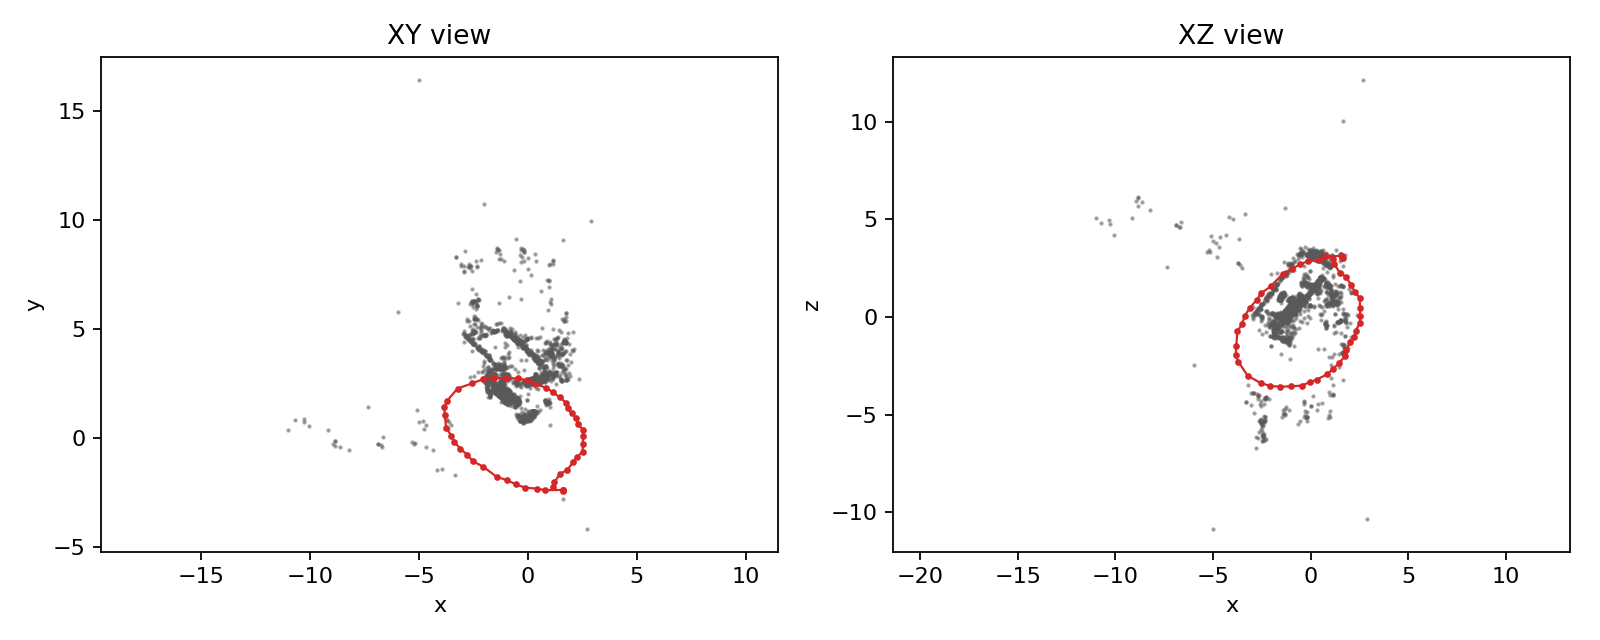
\includegraphics[width=0.95\linewidth]{assets/colmap_geometry.png}
  \caption{COLMAP 训练集稀疏点云与相机轨迹可视化。点云稀疏但相机轨迹连续，说明位姿估计可用。}
  \label{fig:colmap-geometry}
\end{figure}

\subsection{Nerfacto 渲染与深度观察}

图 \ref{fig:nerf-qual} 为 Nerfstudio 导出的测试视角对比图，左侧为真实图像，右侧为 Nerfacto 渲染。Nerfacto 能够恢复讲台、墙面、门框和显示器支架等主要结构，但在细线缆、桌面边缘、椅子局部以及低纹理墙面区域出现明显模糊和噪声。图 \ref{fig:nerf-depth} 的深度结果也显示出边界和反光区域不稳定，说明隐式密度场虽然能表达连续趋势，但几何边界并不总是清晰。

\begin{figure}[H]
  \centering
  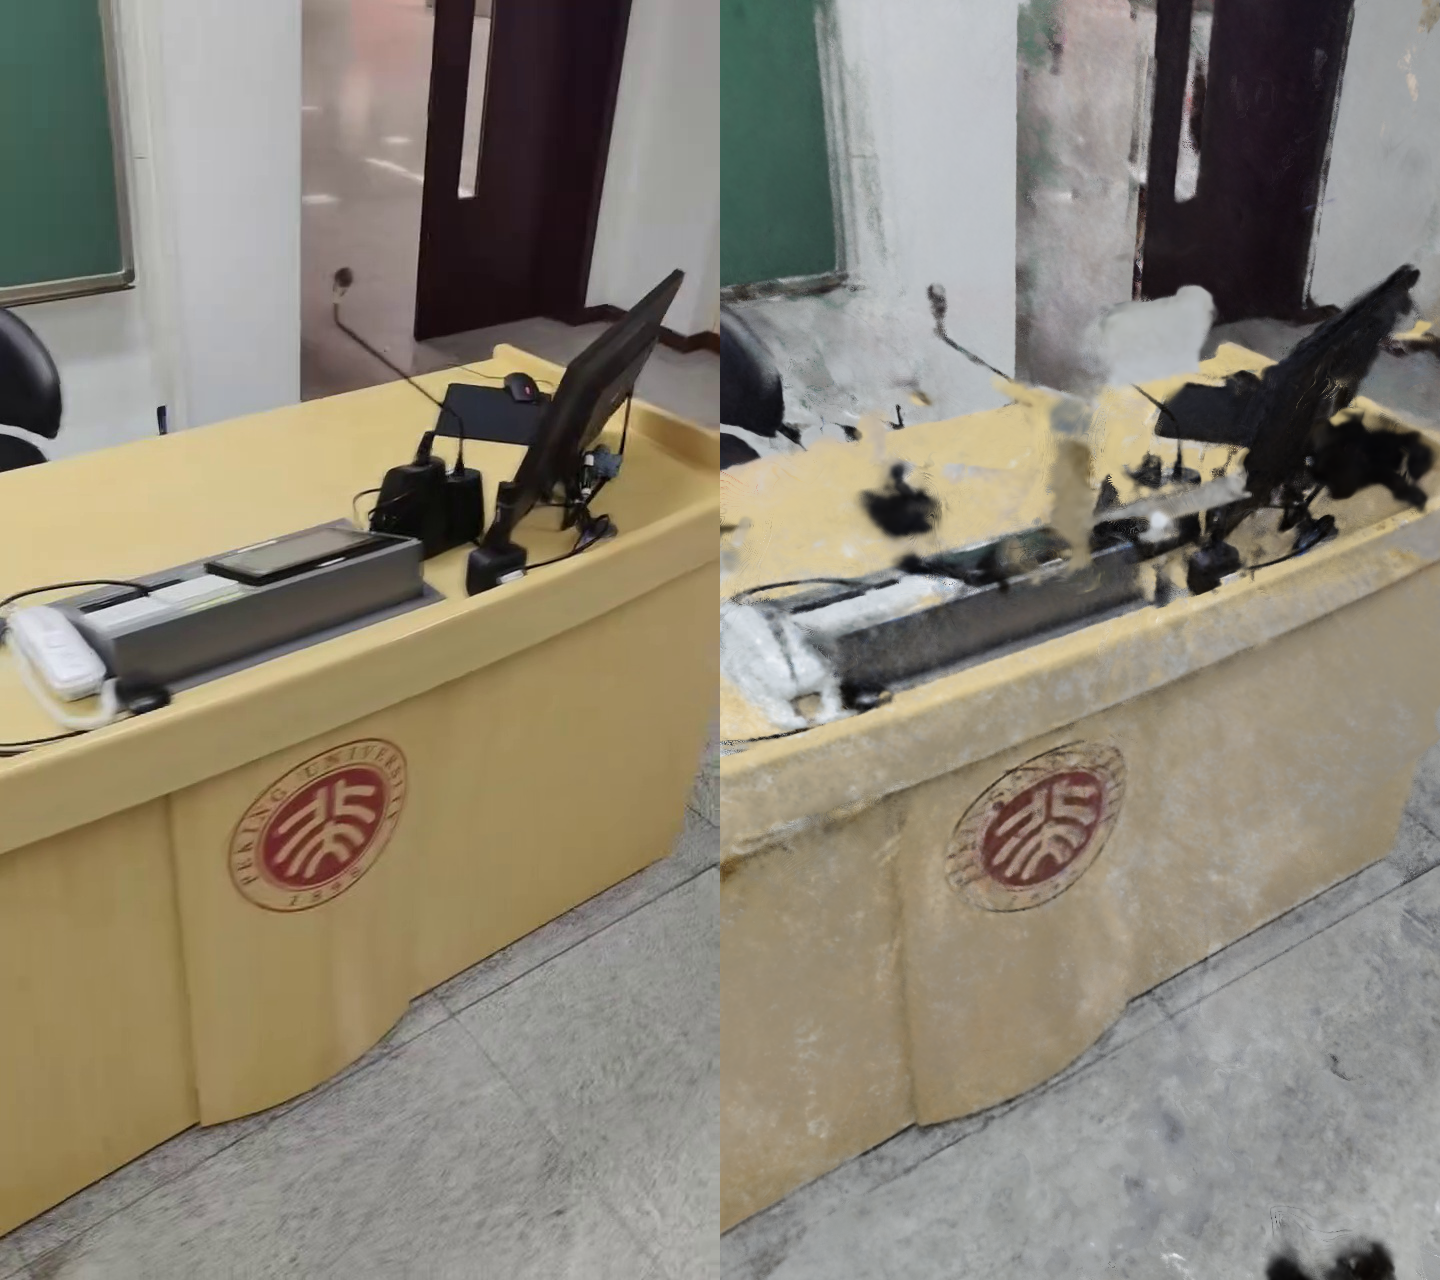
\includegraphics[width=0.82\linewidth]{assets/nerf_eval_img_0000.png}
  \caption{Nerfacto 测试视角定性结果。左侧为真实图像，右侧为渲染结果；整体结构可见，但细节和边界存在模糊。}
  \label{fig:nerf-qual}
\end{figure}

\begin{figure}[H]
  \centering
  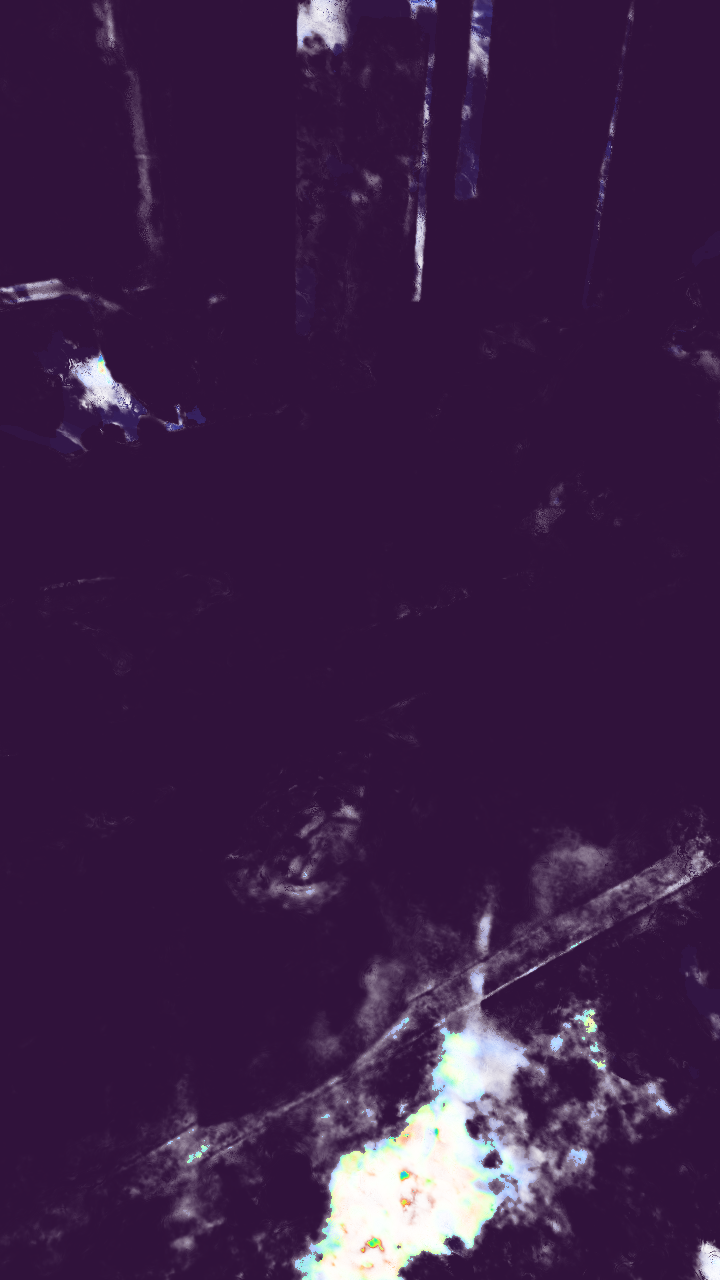
\includegraphics[width=0.42\linewidth]{assets/nerf_depth_0000.png}
  \caption{Nerfacto 导出的深度图。深度可用于观察隐式几何趋势，但低纹理和遮挡边界处噪声较明显。}
  \label{fig:nerf-depth}
\end{figure}

\subsection{3DGS 测试视角渲染}

图 \ref{fig:gs-qual} 展示了 3DGS 在测试视角上的真实图像和渲染结果。相比 Nerfacto，3DGS 的桌面、椅子、黑板边框和墙面纹理更清晰，局部边缘保持更好。这与表 \ref{tab:view-synthesis} 中更高的 PSNR/SSIM 和更低的 LPIPS 一致。

不过，3DGS 的几何仍应谨慎解释。Gaussian 是服务于可微渲染的辐射基元，不是直接重建的网格表面。外观清晰并不意味着几何完全准确，尤其是在遮挡、反光和低纹理区域，Gaussian 可能通过局部不透明度和颜色拟合生成较好的视觉结果，却不对应真实物体表面。

\begin{figure}[H]
  \centering
  \begin{minipage}{0.45\linewidth}
    \centering
    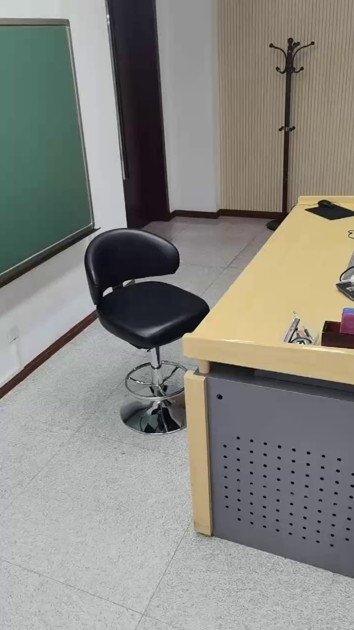
\includegraphics[height=0.37\textheight]{assets/gs_gt_00000.png}
    \caption*{真实图像}
  \end{minipage}
  \hfill
  \begin{minipage}{0.45\linewidth}
    \centering
    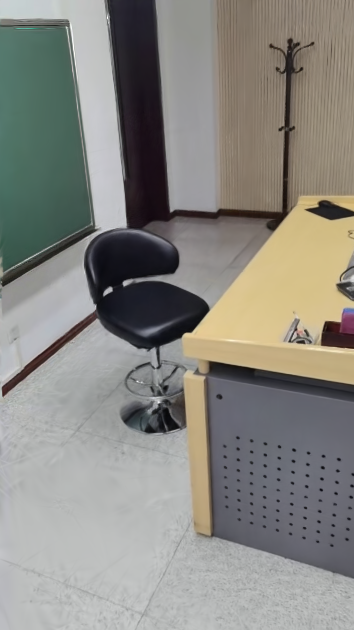
\includegraphics[height=0.37\textheight]{assets/gs_render_00000.png}
    \caption*{3DGS 渲染}
  \end{minipage}
  \caption{3DGS 测试视角定性对比。渲染结果在结构和纹理上接近真实图像。}
  \label{fig:gs-qual}
\end{figure}

\section{讨论}

\subsection{不同表示学到了什么}

COLMAP 学到的是相机位姿、相机内参和可匹配特征对应的稀疏三维点。它保留了几何解释性，但丢掉了大部分外观、材质和低纹理区域的连续表面。对于本实验，COLMAP 最适合作为传统几何基线和后续神经方法的初始化工具。

Nerfacto 学到的是连续隐式辐射场。它能够将同一场景压缩进神经网络参数中，并通过体渲染产生新视角图像。它保留了拓扑灵活性和连续表达能力，但丢掉了直接可编辑的显式结构；在本实验中，有限视角和复杂室内遮挡使其在细节和边界上较弱。

3DGS 学到的是一组显式 Gaussian 辐射基元。它在本实验中最擅长恢复清晰外观和高效渲染，同时比 NeRF 更容易进行局部查看和编辑。但它的几何不是严格表面，Gaussian 的位置和尺度更多服务于图像重建目标，因此不能简单等同于真实三维网格。

\subsection{课程维度比较}

\begin{table}[H]
  \centering
  \caption{三种表示的综合比较}
  \label{tab:discussion}
  \begin{tabular}{p{2.5cm}p{3.5cm}p{3.5cm}p{3.5cm}}
    \toprule
    维度 & COLMAP 稀疏几何 & Nerfacto / NeRF & 3DGS \\
    \midrule
    视觉质量 & 不是完整渲染方法，只提供点云颜色和几何参考 & 整体结构可见，但细节较糊 & 本实验中最清晰，指标最好 \\
    几何质量 & 相机轨迹稳定，点云稀疏且依赖纹理 & 深度连续但边界噪声较多 & 外观几何一致性好，但不是显式表面 \\
    效率 & SfM 很快，约数秒级 & 训练约 5.7 小时，渲染较慢 & 训练约 15 分钟，渲染约 18 秒 \\
    可编辑性 & 点云和相机位姿直观，但表面缺失 & 网络权重难以直接编辑 & Gaussian 基元较易查看和局部调整 \\
    拓扑灵活性 & 依赖稀疏特征点，表达能力有限 & 连续场表达灵活 & 可表达复杂外观，但表面解释有限 \\
    数据采集难度 & 需要纹理和视角重叠 & 需要覆盖充分且姿态可靠 & 同样需要可靠位姿和较密视角 \\
    机器学习集成 & 可作为监督或初始化信号 & 与神经渲染训练天然结合 & 适合实时渲染和可微优化扩展 \\
    \bottomrule
  \end{tabular}
\end{table}

\subsection{失败现象与限制}

本实验的主要限制包括三点。第一，视频时长约 25 s，抽帧只有 51 张，虽然满足基本要求，但对讲台内部遮挡、桌面反光和低纹理墙面覆盖仍有限。第二，不同工具的评估导出视角数量不完全一致，Nerfstudio 和 3DGS 的定量指标只能作为可获得输出下的比较，不能被解释为严格同视角逐像素对比的绝对排名。第三，几何评估缺少真实激光扫描或深度相机真值，因此只能基于 COLMAP 重投影误差、相机轨迹、点云/深度/Gaussian 观察和人眼结构分析进行 proxy 评价。

\section{结论}

本文完成了同一真实室内讲台场景的三种三维表示重建与评估。COLMAP 成功恢复稀疏点云和相机轨迹，是可靠的几何和位姿基线；Nerfacto 能用隐式神经场表达整体场景，但在本实验数据规模下细节和边界质量有限；3DGS 在新视角外观指标、训练效率和渲染效率上表现最好，是本实验中最推荐的视觉重建表示。

如果目标是获得可解释相机位姿和粗略几何，应优先使用 COLMAP；如果目标是研究连续隐式表示和神经渲染机制，NeRF 仍有价值；如果目标是较快获得清晰可交互的新视角渲染，3DGS 更适合当前场景。后续改进方向包括延长采集路径、增加侧向和俯视视角、减少反光区域、加入更严格的共享 hold-out 评估脚本，并可补充 VGGT-GS 作为预训练几何初始化对比。

\appendix
\section{关键复现实验命令}

\begin{verbatim}
python scripts/inspect_video_camera.py
python scripts/prepare_video.py
python scripts/split_dataset.py
python scripts/run_colmap.py
python scripts/analyze_colmap_geometry.py

conda run -n scene-nerf python scripts/run_experiment_suite.py \
  --method nerfstudio --stage train --env-mode fallback
conda run -n scene-nerf python scripts/run_experiment_suite.py \
  --method nerfstudio --stage eval --env-mode fallback

conda run --no-capture-output -n scene-3dgs python \
  external/gaussian-splatting/train.py \
  -s data/3dgs_full_undistorted --images images \
  -m results/3dgs/eval_model --iterations 30000 \
  --resolution 2 --disable_viewer --eval

conda run --no-capture-output -n scene-3dgs python \
  external/gaussian-splatting/render.py \
  -s data/3dgs_full_undistorted --images images \
  -m results/3dgs/eval_model --iteration 30000 --eval

python scripts/evaluate_all.py
python scripts/collect_results.py
\end{verbatim}

\section{主要结果文件}

\begin{itemize}
  \item 定量指标：\texttt{results/metrics.csv}
  \item 运行时间：\texttt{results/timing.csv}
  \item 结果大小：\texttt{results/model\_sizes.csv}
  \item COLMAP 几何摘要：\texttt{results/colmap/train\_geometry\_summary.json}
  \item COLMAP 几何图：\texttt{results/colmap/train\_geometry\_preview.png}
  \item Nerfstudio 评估：\texttt{results/nerfstudio/eval.json}
  \item 3DGS 测试渲染：\texttt{results/3dgs/eval\_model/test/ours\_30000/}
\end{itemize}

\end{document}
